    \documentclass[a4paper,12pt]{article}
    \usepackage[T1]{fontenc}
    \usepackage[polish]{babel}
    \usepackage{amsfonts}
    \usepackage{listings}
    \usepackage{graphicx}
    \usepackage{caption}
    \usepackage{booktabs}
    \usepackage{amssymb}
    \usepackage{amsmath}
    \usepackage[dvipsnames]{xcolor}
    \usepackage[T1]{fontenc}
    \usepackage[utf8]{inputenc}
    \usepackage{subcaption} 
    \usepackage{float}
    \usepackage{geometry}
    \geometry{margin=1in}
    \usepackage{graphicx}
    \usepackage{babel}
    \usepackage{animate}
    \usepackage{hyphenat}
    \usepackage{url} 
    
    \geometry{left=2cm, right=2cm, top=2cm, bottom=2cm}
    
    % Ustawienia dla środowiska lstlisting
    \lstset{ 
      language=Python,
      basicstyle=\footnotesize\ttfamily,
      numbers=left,
      numberstyle=\tiny,
      numbersep=5pt,
      frame=single,
      breaklines=true,
      backgroundcolor=\color{gray!10},
      captionpos=b,
      tabsize=2,
    }
    
    \title{Sprawozdanie z laboratorium 6 - Pierwiastki równań nieliniowych}
    \author{Hubert Miklas}
    \date{06-05-2025}
    
    \begin{document}
    
    \maketitle
    
    \section{Wstęp}
    
    Tematem laboratorium było rozwiązywanie równań i układów równań nieliniowych, korzystając z metod aproksymacji miejsc zerowych funkcji jednej lub wielu zmiennych.
    
    \section{Treści zadań}
    
    \begin{enumerate}
      \item Napisz iterację wg metody Newtona do rozwiązywania każdego z następujących równań nieliniowych:
      \begin{enumerate}
        \item $x \cos(x) = 1$;
        \item $x^3 - 5x - 6 = 0$;
        \item $e^x = x^2 - 1$.
      \end{enumerate}
    
      \item 
      \begin{enumerate}
        \item Pokaż, że iteracyjna metoda matematycznie jest równoważna z metodą siecznych przy rozwiązywaniu skalarnego nieliniowego równania $f(x) = 0$.
        
        \[
        x_{k+1} = \frac{x_{k-1} f(x_k) - x_k f(x_{k-1})}{f(x_k) - f(x_{k-1})}
        \]
    
        \item Jeśli zrealizujemy obliczenia w arytmetyce zmiennoprzecinkowej o skończonej precyzji, jakie zalety i wady ma wzór podany w podpunkcie (a), w porównaniu ze wzorem dla metody siecznych podanym poniżej?
    
        \[
        x_{k+1} = x_k - f(x_k) \cdot \frac{x_k - x_{k-1}}{f(x_k) - f(x_{k-1})}
        \]
      \end{enumerate}
    
      \item Zapisz iterację Newtona do rozwiązywania następującego układu równań nieliniowych:
      \[
      \begin{cases}
      x_1^2 + x_1 x_2^3 = 9 \\
      3 x_1^2 x_2 - x_2^2 = 4
      \end{cases}
      \]
    \end{enumerate}
    
    \section{Metodyka}
    
    Skorzystano z następujących metod:
    \begin{itemize}
        \item Metoda Newtona - Metoda Newtona, inaczej metoda stycznych, jest iteracyjnym algorytmem wyznaczania przybliżonej wartości miejsca zerowego funkcji \(f\), wykorzystującym lokalną liniową aproksymację za pomocą stycznej \cite{wiki:Metoda_Newtona}. Kolejne przybliżenia oblicza się ze wzoru
    \[
      x_{k+1} \;=\; x_k \;-\;\frac{f(x_k)}{f'(x_k)}\,,
    \]
    który otrzymuje się, rozwiązując układ stycznej do wykresu \(f\) w punkcie \((x_k,f(x_k))\) z osią odciętych.
        \item Metoda Netwona dla funkcji wielu zmiennych - Jest to uogólniona metoda Newtona dla rozwiązywania układów równań. Przyjmujemy:
        Dla układu \(F:\mathbb R^n\to\mathbb R^n\) zapis iteracji przyjmuje postać:
    \[
      x_{k+1} \;=\; x_k \;-\;J_F(x_k)^{-1}\,F(x_k)\,,
    \]
    gdzie \(J_F\) to macierz Jacobiego funkcji wektorowej \(F\) \cite{wiki:Metoda_Newtona}
    
    \end{itemize}
    
    \section{Rozwiązania}
    
    \section*{Zadanie 1: Obliczanie miejsc zerowych metodą Newtona dla równań nieliniowych}
    
    Do rozwiązania skorzystamy z metody Newtona opisanej powyżej \cite{wiki:Metoda_Newtona}. 
    
    \paragraph{Założenia}
    Aby metoda zbiegała, powinny być spełnione założenia:
    \begin{enumerate}
      \item \(f\) jest ciągła i ma ciągłą pochodną w otoczeniu pierwiastka,
      \item istnieje dokładnie jedno \(x^*\) takie, że \(f(x^*)=0\),
      \item \(f'(x^*)\neq0\),
      \item punkt startowy \(x_0\) jest dostatecznie blisko \(x^*\).
    \end{enumerate}
    
    \paragraph{Zbieżność}
    Metoda Newtona ma zbieżność kwadratową (rząd 2), co oznacza, że dla wystarczająco bliskiego startu liczba poprawnych cyfr szacunku w przybliżeniu podwaja się każdą iterację \cite{weisstein_newton}.
    
    \subsection{Rozwiązania}
    
    \subsubsection{Równanie (a): $x \cos(x) = 1$}
    
    Funkcja ta będzie miała nieskończenie wiele rozwiązań. Niemniej jednak, jesteśmy w stanie wyznaczyć miejsca zerowe przy zadanych punktach różnych od zera.
    
    Dla równania $x \cos(x) = 1$ przekształcamy je do postaci:
    $f(x) = x \cos(x) - 1 = 0$
    
    Pochodna funkcji to:
    $f'(x) = \cos(x) - x \sin(x)$
    
    Wzór iteracyjny metody Newtona:
    $x_{n+1} = x_n - \frac{x_n \cos(x_n) - 1}{\cos(x_n) - x_n \sin(x_n)}$
    
    \subsubsection{Równanie (b): $x^3 - 5x - 6 = 0$}
    
    Dla równania wielomianowego $x^3 - 5x - 6 = 0$, definiujemy:
    $f(x) = x^3 - 5x - 6$
    
    Pochodna:
    $f'(x) = 3x^2 - 5$
    
    Wzór Newtona:
    $x_{n+1} = x_n - \frac{x_n^3 - 5x_n - 6}{3x_n^2 - 5}$
    
    \subsubsection{Równanie (c): $e^{-x} = x^2 - 1$}
    
    Równanie przekształcamy do postaci:
    $f(x) = e^{-x} - x^2 + 1 = 0$
    
    Pochodna funkcji:
    $f'(x) = -e^{-x} - 2x$
    
    Wzór iteracyjny:
    $x_{n+1} = x_n - \frac{e^{-x_n} - x_n^2 + 1}{-e^{-x_n} - 2x_n}$
    
    \subsubsection{Analiza zbieżności}
    
    Metoda Newtona zbiega kwadratowo, gdy spełnione są następujące warunki:
    \begin{enumerate}
        \item Funkcja $f$ jest ciągle różniczkowalna
        \item Pierwiastek $r$ jest prosty ($f'(r) \neq 0$)
        \item Początkowe przybliżenie $x_0$ jest dostatecznie blisko $r$
    \end{enumerate}
    
    Dla naszych równań zbieżność wygląda następująco:
    
    \subsubsection{Dla $x \cos(x) = 1$}
    Kod znalazł pierwiastek w pobliżu $x \approx 4.9171859253$ i  $x \approx 36.1559769881$. Metoda Newtona zwykle szybko zbiega przy początkowym przybliżeniu z przedziału $[0, 1]$. Jednakże pochodna może zanikać dla pewnych wartości $x$ i dużej dokładności (tj. bardzo małej wartości) $\epsilon$, co jest spowodowane dużą liczbą iteracji. Miejsce zerowe $x \approx 36.1559769881$ zostało znalezione dla wartości $x_0 = 1.0$ dla precyzji $\epsilon = 10^{-14}$, co sugeruje, że właśnie taki problem wystąpił.
    
    \begin{figure}[H]
        \centering
        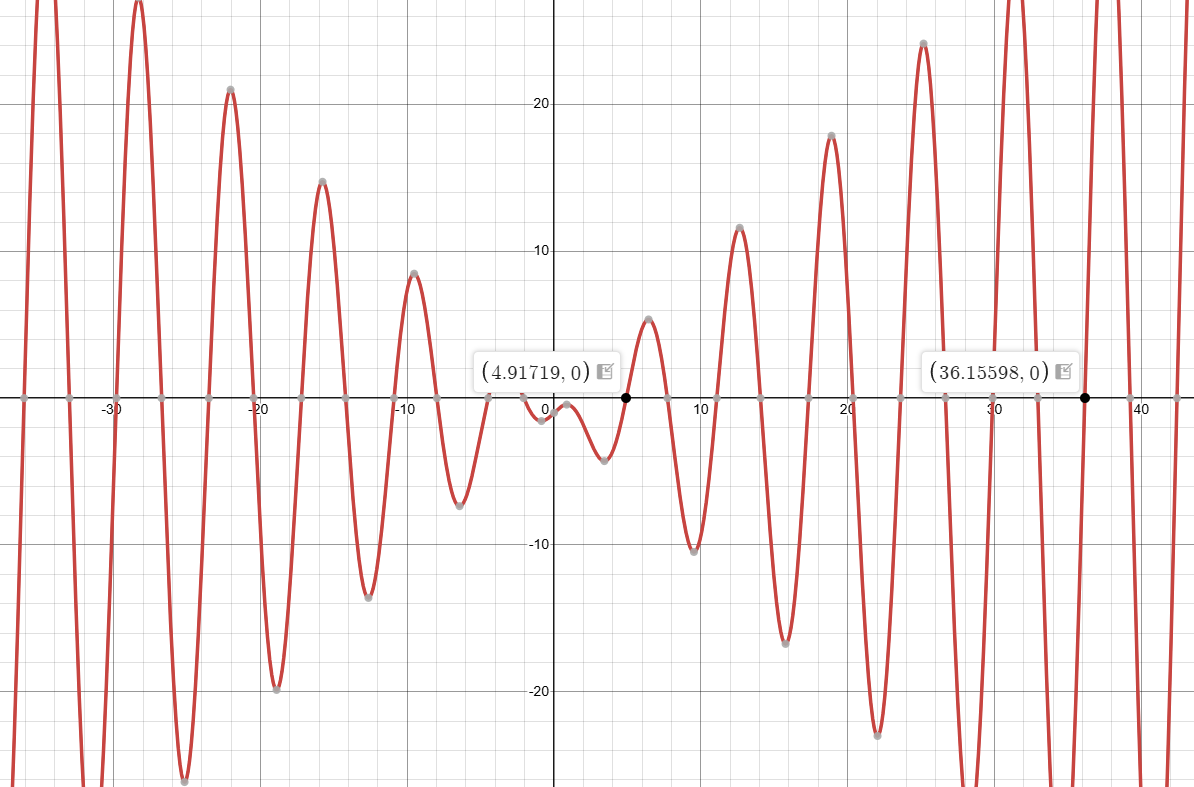
\includegraphics[width=1\linewidth]{found_points.PNG}
        \caption{Dwa znalezione miejsca zerowe dla równania $x \cdot \cos x = 1$. Widać, że istnieje ich nieskończenie wiele, jednak w tym przypadku algorytm Netwona schodzi do pewnego wybranego punktu.}
        \label{fig:first-solutions}
    \end{figure}
    
    \subsubsection{Dla $x^3 - 5x - 6 = 0$}
    Wielomian ten ma pierwiastki rzeczywiste w $x \approx 2.6890953236 $ i zespolone w $x \approx \pm \sqrt{\frac{5}{3}}i$. Metoda Newtona działa bardzo dobrze dla wielomianów i szybko zbiega do $x \approx 3$ przy rozsądnym starcie, np. $x_0 = 2$.
    
    \begin{figure}[H]
        \centering
        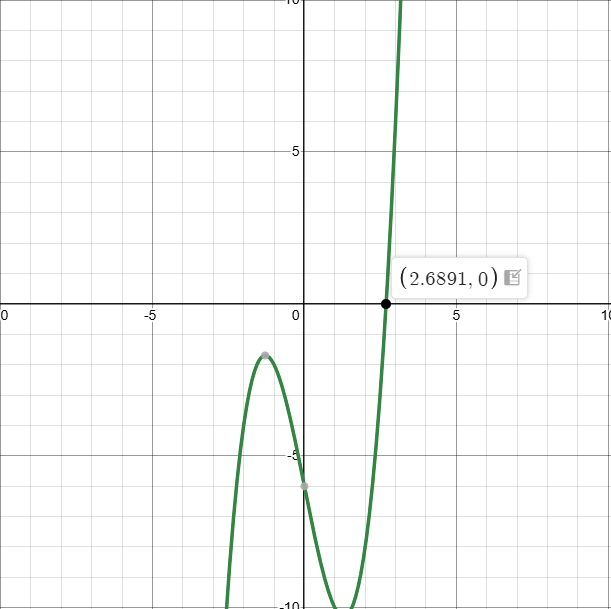
\includegraphics[width=0.7\linewidth]{second_solution.PNG}
        \caption{Znalezione miejsce zerowe na wykresie}
        \label{fig:first-solutions}
    \end{figure}
    
    \subsubsection{Dla $e^{-x} = x^2 - 1$}
    Równanie to łączy składniki wykładnicze i wielomianowe. Ma pierwiastki w pobliżu $x \approx 1.1477576321$. Wybór odpowiedniego przybliżenia początkowego jest kluczowy dla zbieżności do żądanego pierwiastka.
    
    \begin{figure}[H]
        \centering
        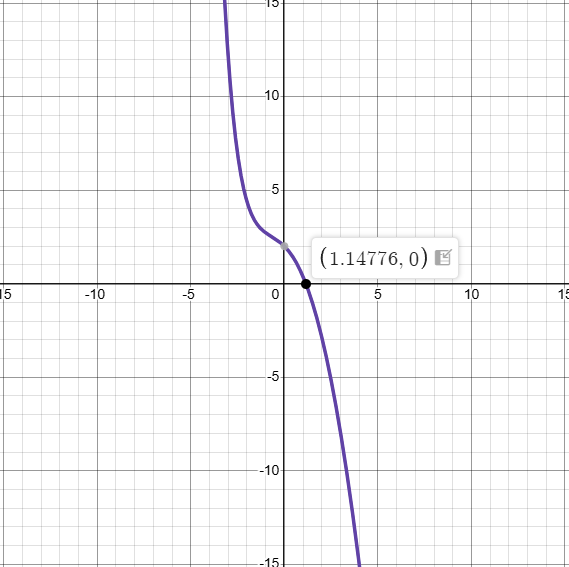
\includegraphics[width=0.7\linewidth]{third_solution.PNG}
        \caption{Znalezione miejsce zerowe na wykresie}
        \label{fig:third-solution}
    \end{figure}
    
    \subsubsection{Uwagi dotyczące implementacji praktycznej}
    
    W implementacji w języku Python uwzględniono następujące zabezpieczenia:
    \begin{itemize}
        \item Ochrona przed dzieleniem przez pochodne bliskie zeru
        \item Ograniczenie liczby iteracji, aby uniknąć nieskończonej pętli
        \item Parametr tolerancji ($\epsilon$) kontrolujący precyzję zbieżności
        \item Wiele punktów startowych, aby zwiększyć szansę znalezienia wszystkich pierwiastków
    \end{itemize}
    
    \newpage
    
    \subsection{Kod w Python-ie iustrujący obliczenia}
    
    \begin{lstlisting}
    from numpy import cos, sin, exp
    import matplotlib.pyplot as plt
    import numpy as np
    
    def newton_approx(f=lambda x: x, f_der=lambda x: 1, x0=1.0, epsilon=1e-16, max_iter=100):
        x = x0
        iterations = 0
        while abs(f(x)) > epsilon and iterations < max_iter:
            if abs(f_der(x)) < 1e-10:
                raise ValueError("Derivative too close to zero - divergent")
            x = x - f(x)/f_der(x)
            iterations += 1
        return x, iterations
    
    def f1(x):
        return x * cos(x) - 1
    
    def f1_der(x):
        return cos(x) - x * sin(x)
    
    def f2(x):
        return x**3 - 5*x - 6
    
    def f2_der(x):
        return 3 * x**2 - 5
    
    def f3(x):
        return exp(-x) - x**2 + 1
    
    def f3_der(x):
        return -exp(-x) - 2*x
    
    def compare_methods(f, f_der, x0_values, epsilon_values, title):
        results = []
        for x0 in x0_values:
            for eps in epsilon_values:
                try:
                    root, iterations = newton_approx(f, f_der, x0, eps)
                    results.append({
                        'x0': x0,
                        'epsilon': eps,
                        'root': root,
                        'iterations': iterations,
                        'final_error': abs(f(root))
                    })
                except ValueError as e:
                    print(f"Error with x0={x0}, epsilon={eps}: {e}")
    
        # Print results in a table format
        print(f"\nResults for {title}:")
        print(f"{'x0':^10} | {'epsilon':^12} | {'root':^15} | {'iterations':^10} | {'final error':^12}")
        print("-" * 65)
        for r in results:
            print(f"{r['x0']:^10} | {r['epsilon']:^12.1e} | {r['root']:^15.10f} | {r['iterations']:^10} | {r['final_error']:^12.2e}")
        return results
    
    def get_different_roots(results, epsilon=1e-4):
        roots = [] 
        for element in results:
            root = element['root']
            if len(roots) == 0:
                roots.append(root)
            for other in roots:
                if abs(root - other) > epsilon:
                    roots.append(root)
        return roots
    \end{lstlisting}
    
    \subsubsection{Wnioski}
    
    Metoda Newtona jest skuteczną techniką rozwiązywania równań nieliniowych, szczególnie gdy dostępne są dobre przybliżenia początkowe. W sprzyjających warunkach metoda wykazuje zbieżność kwadratową, co czyni ją znacznie szybszą niż prostsze metody, np. metoda bisekcji.
    
    \begin{enumerate}
    \item Dla trzech analizowanych równań:
    \begin{enumerate}
        \item $x \cos(x) = 1$ ma rozwiązanie w $x \approx 4.9171859253$ i  $x \approx 36.1559769881$ 
        \item $x^3 - 5x - 6 = 0$ ma rozwiązanie przy $x \approx 2.6890953236 $, ze na to, że jest to równanie sześcienne, można je rozwiązać analitycznie \cite{wiki:Cubic_equation} 
        \item $e^{-x} = x^2 - 1$ ma rozwiązania przy 
    \end{enumerate}
    \end{enumerate}
    
    Wszystkie te rozwiązania mogą być efektywnie znalezione metodą Newtona przy odpowiednich przybliżeniach początkowych.
    
    \section*{Zadanie 2: Dowód i analiza uogólnionego wzoru Newtona}
    
    \subsection*{(a) Równoważność z metodą siecznych}
    
    Metoda siecznych dla równania \(f(x)=0\) jest dana iteracją
    \[
    x_{k+1}
    \;=\;
    x_k - f(x_k)\,\frac{x_k - x_{k-1}}{f(x_k)-f(x_{k-1})}.
    \]
    Przekształćmy tę formułę:
    \[
    x_{k+1}
    =
    \frac{x_k\bigl(f(x_k)-f(x_{k-1})\bigr)
          -f(x_k)\,(x_k-x_{k-1})}
         {f(x_k)-f(x_{k-1})} \Rightarrow
    \]
    \[
    \frac{x_k\bigl(f(x_k)-f(x_{k-1})\bigr)
          -f(x_k)\,(x_k-x_{k-1})}
         {f(x_k)-f(x_{k-1})}
    =
    \frac{x_kf(x_k)-x_kf(x_{k-1})-x_kf(x_k)+x_{k-1}f(x_k)}
         {f(x_k)-f(x_{k-1})} \Rightarrow
    \]
    \[
    \frac{x_kf(x_k)-x_kf(x_{k-1})-x_kf(x_k)+x_{k-1}f(x_k)}
         {f(x_k)-f(x_{k-1})}
    =
    \frac{x_{k-1}f(x_k)-x_kf(x_{k-1})}{f(x_k)-f(x_{k-1})},
    \]
    
    co dokładnie daje formułę podaną w zadaniu.
    
    \subsection*{(b) Numeryczna analiza wzoru}
    
    W arytmetyce zmiennoprzecinkowej o skończonej precyzji:
    
    \begin{itemize}
      \item \textbf{Zalety formy}
        \begin{itemize}
          \item Unika mnożenia małych różnic typu \((x_k - x_{k-1})\), przenosząc je pod jeden ułamek.
          \item Może zmniejszać lokalne wzmocnienie błędu, gdy \(f(x_k)\approx f(x_{k-1})\).
        \end{itemize}
      \item \textbf{Wady formy}
        \begin{itemize}
          \item Więcej operacji mnożenia i odejmowania – większe ryzyko akumulacji zaokrągleń.
          \item Gdy \(f(x_k)-f(x_{k-1})\) jest bardzo małe, nadal dzielimy przez małą liczbę, co może prowadzić do znacznych błędów.
        \end{itemize}
      \item \textbf{W praktyce} zwykle stosuje się pierwotny zapis
      \(\;x_{k+1}=x_k - f(x_k)\frac{x_k - x_{k-1}}{f(x_k)-f(x_{k-1})}\),
      który jest nieco prostszy i często równie stabilny.ac
    \end{itemize}
    
    \section*{Zadanie 3: Rozwiązanie nieliniowego układu równań uogólnioną metodą Newtona}
    
    Dana jest funkcja wektorowa
    \[
    \mathbf{F}(x_1,x_2)
    =\begin{pmatrix}
    f_1(x_1,x_2)\\[6pt]
    f_2(x_1,x_2)
    \end{pmatrix}
    =
    \begin{pmatrix}
    x_1^2 + x_1 x_2^3 - 9 \\[4pt]
    3x_1^2 x_2 - x_2^3 - 4
    \end{pmatrix}.
    \]
    Macierz Jacobiego \(J = \bigl(\partial f_i/\partial x_j\bigr)\) ma postać
    \[
    J(x_1,x_2)
    =
    \begin{pmatrix}
    2x_1 + x_2^3 & 3x_1\,x_2^2\\[6pt]
    6x_1\,x_2   & 3x_1^2 - 3x_2^2
    \end{pmatrix}.
    \]
    Iteracja Newtona wyraża się wzorem
    \[
    \begin{aligned}
    J\bigl(x^{(k)}\bigr)\,\Delta x^{(k)}
    &= -\,\mathbf{F}\bigl(x^{(k)}\bigr),\\
    x^{(k+1)} &= x^{(k)} + \Delta x^{(k)},
    \end{aligned}x
    \]
    czyli jawnie
    \[
    x^{(k+1)}
    =
    x^{(k)}
    - J\bigl(x^{(k)}\bigr)^{-1}\,\mathbf{F}\bigl(x^{(k)}\bigr).
    \]
    
    
    \subsection*{Kroki obliczeń}
    
    Korki obliczeń wykonane przez komputer prezentują się następująco:
    
    \begin{enumerate}
    \item Punkt wyjściowy: $x_0 = 1.500000$, $y_0 = 1.000000$
    \item Iteracja 1:
      \begin{itemize}
        \item Punkt: $(x_0, y_0) = (1.500000, 1.000000)$
        \item Wartości funkcji: $F(x,y) = [-5.250000, 1.750000]^T$
        \item $||F(x,y)|| = 5.533986e+00$
        \item Macierz Jakobiego: $J = \begin{bmatrix} 4.000000 & 4.500000 \\ 9.000000 & 3.750000 \end{bmatrix}$
        \item $\Delta = [-1.080882, 2.127451]^T$
        \item Następny punkt: $(x_1, y_1) = (0.419118, 3.127451)$
      \end{itemize}
    \item Iteracja 2:
      \begin{itemize}
        \item Punkt: $(x_1, y_1) = (0.419118, 3.127451)$
        \item Wartości funkcji: $F(x,y) = [3.996234, -32.941340]^T$
        \item $||F(x,y)|| = 3.318285e+01$
        \item Macierz Jakobiego: $J = \begin{bmatrix} 31.427676 & 12.298106 \\ 7.864619 & -28.815870 \end{bmatrix}$
        \item $\Delta = [0.289285, -1.064213]^T$
        \item Następny punkt: $(x_2, y_2) = (0.708403, 2.063238)$
      \end{itemize}
    \item Iteracja 3:
      \begin{itemize}
        \item Punkt: $(x_2, y_2) = (0.708403, 2.063238)$
        \item Wartości funkcji: $F(x,y) = [-2.276187, -9.676890]^T$
        \item $||F(x,y)|| = 9.940987e+00$
        \item Macierz Jakobiego: $J = \begin{bmatrix} 10.199910 & 9.046912 \\ 8.769625 & -11.265350 \end{bmatrix}$
        \item $\Delta = [0.582712, -0.405378]^T$
        \item Następny punkt: $(x_3, y_3) = (1.291115, 1.657860)$
      \end{itemize}
    \item Iteracja 4:
      \begin{itemize}
        \item Punkt: $(x_3, y_3) = (1.291115, 1.657860)$
        \item Wartości funkcji: $F(x,y) = [-1.449893, -0.265782]^T$
        \item $||F(x,y)|| = 1.474053e+00$
        \item Macierz Jakobiego: $J = \begin{bmatrix} 7.138857 & 10.645886 \\ 12.842925 & -3.244567 \end{bmatrix}$
        \item $\Delta = [0.047119, 0.104596]^T$
        \item Następny punkt: $(x_4, y_4) = (1.338234, 1.762456)$
      \end{itemize}
    \item Iteracja 5:
      \begin{itemize}
        \item Punkt: $(x_4, y_4) = (1.338234, 1.762456)$
        \item Wartości funkcji: $F(x,y) = [0.117206, -0.005638]^T$
        \item $||F(x,y)|| = 1.173414e-01$
        \item Macierz Jakobiego: $J = \begin{bmatrix} 8.151097 & 12.470671 \\ 14.151471 & -3.946139 \end{bmatrix}$
        \item $\Delta = [-0.001880, -0.008170]^T$
        \item Następny punkt: $(x_5, y_5) = (1.336354, 1.754286)$
      \end{itemize}
    \item Iteracja 6:
      \begin{itemize}
        \item Punkt: $(x_5, y_5) = (1.336354, 1.754286)$
        \item Wartości funkcji: $F(x,y) = [0.000618, -0.000210]^T$
        \item $||F(x,y)|| = 6.524147e-04$
        \item Macierz Jakobiego: $J = \begin{bmatrix} 8.071557 & 12.337968 \\ 14.066086 & -3.875028 \end{bmatrix}$
        \item $\Delta = [0.000001, -0.000051]^T$
        \item Następny punkt: $(x_6, y_6) = (1.336355, 1.754235)$
      \end{itemize}
    \item Iteracja 7:
      \begin{itemize}
        \item Punkt: $(x_6, y_6) = (1.336355, 1.754235)$
        \item Wartości funkcji: $F(x,y) = [0.000000, -0.000000]^T$
        \item $||F(x,y)|| = 2.245655e-08$
        \item Macierz Jakobiego: $J = \begin{bmatrix} 8.071091 & 12.337264 \\ 14.065690 & -3.874486 \end{bmatrix}$
        \item $\Delta = [0.000000, -0.000000]^T$
        \item Następny punkt: $(x_7, y_7) = (1.336355, 1.754235)$
      \end{itemize}
    \item Iteracja 8:
      \begin{itemize}
        \item Punkt: $(x_7, y_7) = (1.336355, 1.754235)$
        \item Wartości funkcji: $F(x,y) = [0.000000, 0.000000]^T$
        \item $||F(x,y)|| = 3.552714e-15$
        \item Macierz Jakobiego: $J = \begin{bmatrix} 8.071091 & 12.337264 \\ 14.065690 & -3.874486 \end{bmatrix}$
        \item $\Delta = [-0.000000, -0.000000]^T$
        \item Następny punkt: $(x_8, y_8) = (1.336355, 1.754235)$
      \end{itemize}
    \item Iteracja 9:
      \begin{itemize}
        \item Punkt: $(x_8, y_8) = (1.336355, 1.754235)$
        \item Wartości funkcji: $F(x,y) = [0.000000, 0.000000]^T$
        \item $||F(x,y)|| = 0.000000e+00$
        \item Macierz Jakobiego: $J = \begin{bmatrix} 8.071091 & 12.337264 \\ 14.065690 & -3.874486 \end{bmatrix}$
        \item Warunek zbieżności: $||F(x,y)|| < 1e-16$
      \end{itemize}
    \end{enumerate}
     
     Jak widać na rysunku \ref{fig:task_three}, aby wygenerować wszystkie rozwiązania, należy wybrać parę punktów przykład leżących na okręgu oznaczonego na rysunku następnie skorzystać z algorytmu Metody Newtona i odfilrować powtarzające się (z zadaną precyzją) punkty.
    
    \begin{figure}[H]
        \centering
        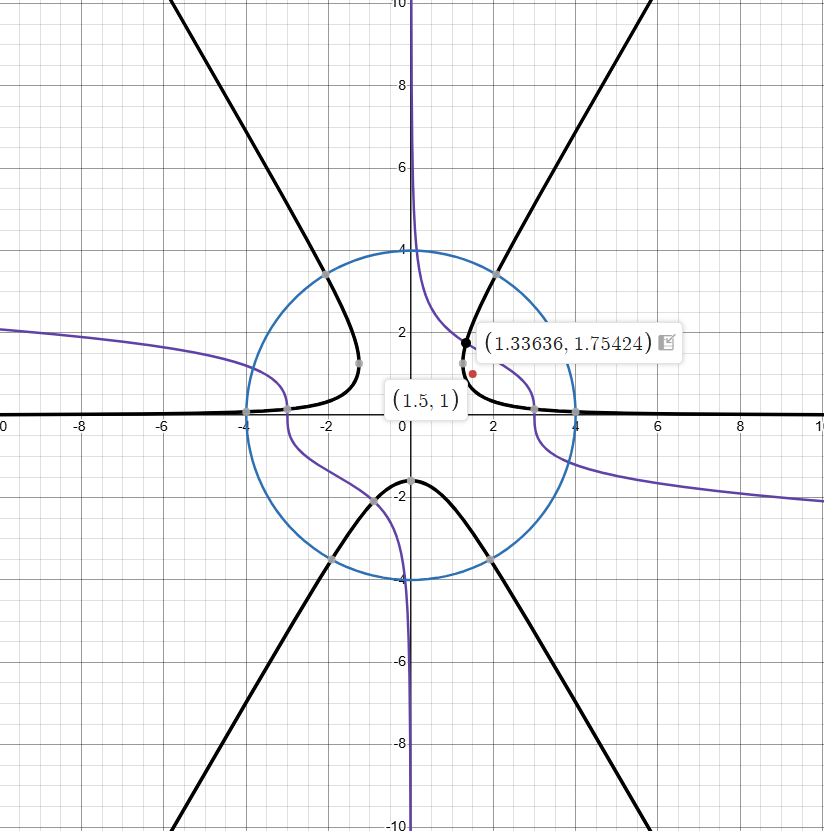
\includegraphics[width=1\linewidth]{task_three.PNG}
        \caption{Znalezione rozwiązanie z punktem początkowym.}
        \label{fig:task_three}
    \end{figure}
    
    Kod do programu generującego wszystkie kroki zamieszczam poniżej.
    
    
    \subsection*{Kod w Pythonie ilustrujący obliczenia}
    
    \begin{lstlisting}
        import numpy as np
    
    def first_function(x, y):
        return x ** 2 + x * y ** 3 - 9 
            
    def first_function_der_x(x, y):
        return 2 * x + y ** 3 
    
    def first_function_der_y(x, y):
        return 3 * x * y ** 2
    
    def second_function(x, y):
        return 3 * x ** 2 * y - y ** 3 - 4
    
    def second_function_der_x(x, y):
        return 6 * x * y
    
    def second_function_der_y(x, y):
        return 3 * x ** 2 - 3 * y ** 2
    
    def make_jacobian(x, y):
        return np.array([
            [first_function_der_x(x, y), first_function_der_y(x, y)],
            [second_function_der_x(x, y), second_function_der_y(x, y)]
        ])
    
    def make_vector(x, y):
        return np.array([first_function(x, y), second_function(x, y)])
    
    def newton_method(x0, y0, tol=1e-16, max_iter=20):
        x, y = x0, y0
        print("\\begin{enumerate}")
        print(f"\\item Punkt wyjściowy: $x_0 = {x0:.6f}$, $y_0 = {y0:.6f}$")
        for iteration in range(max_iter):
            F = make_vector(x, y)
            f_norm = np.linalg.norm(F)
            J = make_jacobian(x, y)
            print(f"\\item Iteracja {iteration + 1}:")
            print(f"  \\begin{{itemize}}")
            print(f"    \\item Punkt: $(x_{iteration}, y_{iteration}) = ({x:.6f}, {y:.6f})$")
            print(f"    \\item Wartości funkcji: $F(x,y) = [{F[0]:.6f}, {F[1]:.6f}]^T$")
            print(f"    \\item $||F(x,y)|| = {f_norm:.6e}$")
            print(f"    \\item Macierz Jakobiego: $J = \\begin{{bmatrix}} {J[0,0]:.6f} & {J[0,1]:.6f} \\\\ {J[1,0]:.6f} & {J[1,1]:.6f} \\end{{bmatrix}}$")
            if f_norm < tol:
                print(f"    \\item Warunek zbieżności: $||F(x,y)|| < {tol}$")
                print(f"  \\end{{itemize}}")
                print("\\end{enumerate}")
                return x, y, iteration, True
            try:
                delta = np.linalg.solve(J, -F)
                print(f"    \\item $\\Delta = [{delta[0]:.6f}, {delta[1]:.6f}]^T$")
                x += delta[0]
                y += delta[1]
                print(f"    \\item Następny punkt: $(x_{iteration+1}, y_{iteration+1}) = ({x:.6f}, {y:.6f})$")
                print(f"  \\end{{itemize}}")
            except np.linalg.LinAlgError:
                print(f"    \\item Macierz z zerowym wyznacznikiem - rozbieżność")
                print(f"  \\end{{itemize}}")
                print("\\end{enumerate}")
                return x, y, iteration, False
        return x, y, max_iter, False
    
    if __name__ == "__main__":
        x0, y0 = 1.5, 1.0
        x_sol, y_sol, iterations, converged = newton_method(x0, y0)
        if converged:
            print(f"\n% Summary")
            print(f"% Solution found after {iterations + 1} iterations:")
            print(f"% x = {x_sol:.10f}, y = {y_sol:.10f}")
            print(f"% Function values at solution:")
            print(f"% f1(x,y) = {first_function(x_sol, y_sol):.10e}")
            print(f"% f2(x,y) = {second_function(x_sol, y_sol):.10e}")
        else:
            print(f"\n% Failed to converge after {iterations + 1} iterations.")
            print(f"% Last values: x = {x_sol:.10f}, y = {y_sol:.10f}")
    
    \end{lstlisting}
    
    
    \subsection*{Wnioski}
    
    \begin{enumerate}
      \item Metoda Newtona dla badanego układu nieliniowego zbiega bardzo szybko — w naszym przykładzie dostateczną precyzję osiągnięto już po 9 iteracjach, mimo początkowo dalekiego od rozwiązania punktu startowego.
      \item Tempo zbieżności jest kwadratowe pod warunkiem, że macierz Jacobiego w pobliżu rozwiązania pozostaje nieosobliwa. Widzimy to wyraźnie w gwałtownym spadku normy wektora funkcji \(\|\mathbf F(x^{(k)})\|\) od kroku 4 w dół.
      \item Poprawny dobór punktu początkowego ma kluczowe znaczenie — przy innych punktach startowych możliwe byłyby zbieżność do innego rozwiązania lub brak zbieżności. Dlatego, aby uzyskać wszystkie rozwiązania układu, należy spróbować kilku różnych punktów startowych na wybranym obszarze (np. na okręgu pokazanym na rysunku \ref{fig:task_three}).
      \item Obliczanie i odwracanie macierzy Jacobiego w każdym kroku generuje istotny koszt obliczeniowy, co przy dużych układach mogłoby stać się wąskim gardłem. W praktyce można rozważyć modyfikacje metody Newtona (np. metody quasi-Newtona) lub przyspieszenie rozwiązywania układów liniowych.
      \item Metoda okazała się stabilna wobec małych zakłóceń — po osiągnięciu obszaru lokalnej zbieżności kolejne poprawki \(\Delta x^{(k)}\) są coraz mniejsze, aż do osiągnięcia granicy precyzji maszynowej.
    \end{enumerate}
    
    
    \bibliographystyle{plain}
    \bibliography{references}
    
    \end{document}
    
